\section{Preliminaries}

\textbf{Group Relative Policy Optimization} \citep[\textbf{GRPO},][]{GRPO}.
GRPO removes the separate critic model in Proximal Policy Optimization \citep[PPO,][]{PPO} to enhance training efficiency.
Given a QA pair $(x,a)$ from the dataset $\mathcal D$, it generates a response group $G=\{y_i\}_{i=1}^{|G|}$ using the current policy $\pi_{\theta_\text{old}}$, computes corresponding rewards $\{R_i\}_{i=1}^{|G|}$, and estimates the advantage via:
\begin{equation}\label{eqn:advantage}
    \hat A_{i,t} = \frac{R_i - \mathrm{mean}(\{R_i\}_{i=1}^{|G|})}{\mathrm{std}(\{R_i\}_{i=1}^{|G|})}.
\end{equation}

The policy $\pi_\theta$ is then optimized by maximizing $\mathcal J_\text{GRPO}(\theta)$, defined as:
\begin{gather*}%\label{eqn:GRPO}
   \mathcal J =\mathbb E_{
    \mathmakebox[4em][r]{
        \substack{ 
        \hspace{2em}(x,a)\sim\mathcal{D}\\
        \{y_i\}_{i=1}^{|G|} \sim\pi_{\theta_{\text{old}}}(\cdot|x)
        }
    }}\bigg[
     \frac{1}{|G|}\sum_{i=1}^{|G|}\frac{1}{|y_i|}\sum_{t=1}^{|y_i|}\min \Bigl( r_{i,t}(\theta)\hat{A}_{i,t}, \notag \\
    \;\;  \text{clip}\bigl(r_{i,t}(\theta), 1-\epsilon, 1+\epsilon\bigr)\hat{A}_{i,t} \Bigr) - \beta\mathbb D_\mathrm{KL}(\pi_\theta\|\pi_\mathrm{ref}) \bigg],
\end{gather*}
where $r_{i,t}(\theta) = \frac{\pi_{\theta}(y_{i,t}|x, y_{i,<t})}{\pi_{\theta_{\text{old}}}(y_{i,t}|x, y_{i,<t})}$ denotes the importance sampling ratio with $1\pm\epsilon$ being the clipping range, and the KL penalty  $\mathbb D_\mathrm{KL}(\pi_\theta\|\pi_\mathrm{ref})$ regularizes the policy towards the reference policy $\pi_\mathrm{ref}$.

\noindent\textbf{Dynamic Sampling Policy Optimization} \citep[\textbf{DAPO},][]{DAPO}. DAPO is a prominent critic-free RL algorithm that further refines GRPO. 
It employs token-level loss aggregation and introduces the clip-higher mechanism with two clip range of  $\epsilon_\text{low}, \epsilon_\text{high}$, while removing the KL penalty:
\begin{gather}\label{eqn:DAPO}
   \mathcal J_\text{DAPO}(\theta) = \mathbb E_{
    \mathmakebox[4em][r]{
        \substack{ 
        \hspace{2em}(x,a)\sim\mathcal{D}\\
        \{y_i\}_{i=1}^{|G|} \sim\pi_{\theta_{\text{old}}}(\cdot|x)
        }
    }}\bigg[
     \frac{1}{\sum_{i=1}^{|G|} |y_i|} \sum_{i=1}^{|G|} \sum_{t=1}^{|y_i|}  \\
    \min \Bigl( r_{i,t}(\theta)\hat{A}_{i,t}, \text{clip}\bigl(r_{i,t}(\theta), 1-\epsilon_\text{low}, 1+\epsilon_\text{high}\bigr)\hat{A}_{i,t} \Bigr) \bigg],\notag
\end{gather}
Moreover, DAPO employs a dynamic sampling strategy to ensure the response group is not all correct or all wrong:
$$
0 < \left|\{y_i \mid \text{is\_equivalent}(a, y_i)\}\right| < {|G|}
$$
Given its established efficacy, we adopt DAPO as the primary baseline for our empirical analysis.

\begin{figure*}[t]
    \centering
    \begin{subfigure}[b]{0.377\linewidth}
        \centering
        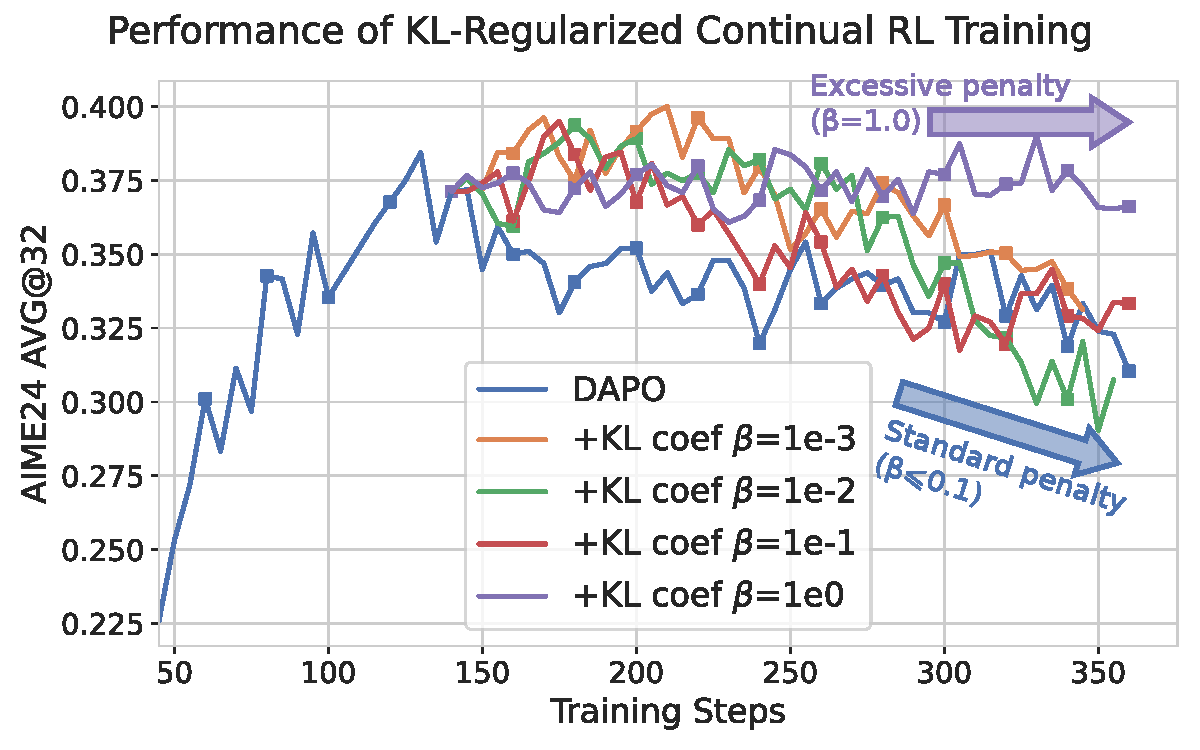
\includegraphics[width=\linewidth]{figs/different_kl.pdf}
        \caption{KL regularized validation performance}
        \label{fig:kl_perf}
    \end{subfigure}
    \hfill
    \begin{subfigure}[b]{0.377\linewidth}
        \centering
        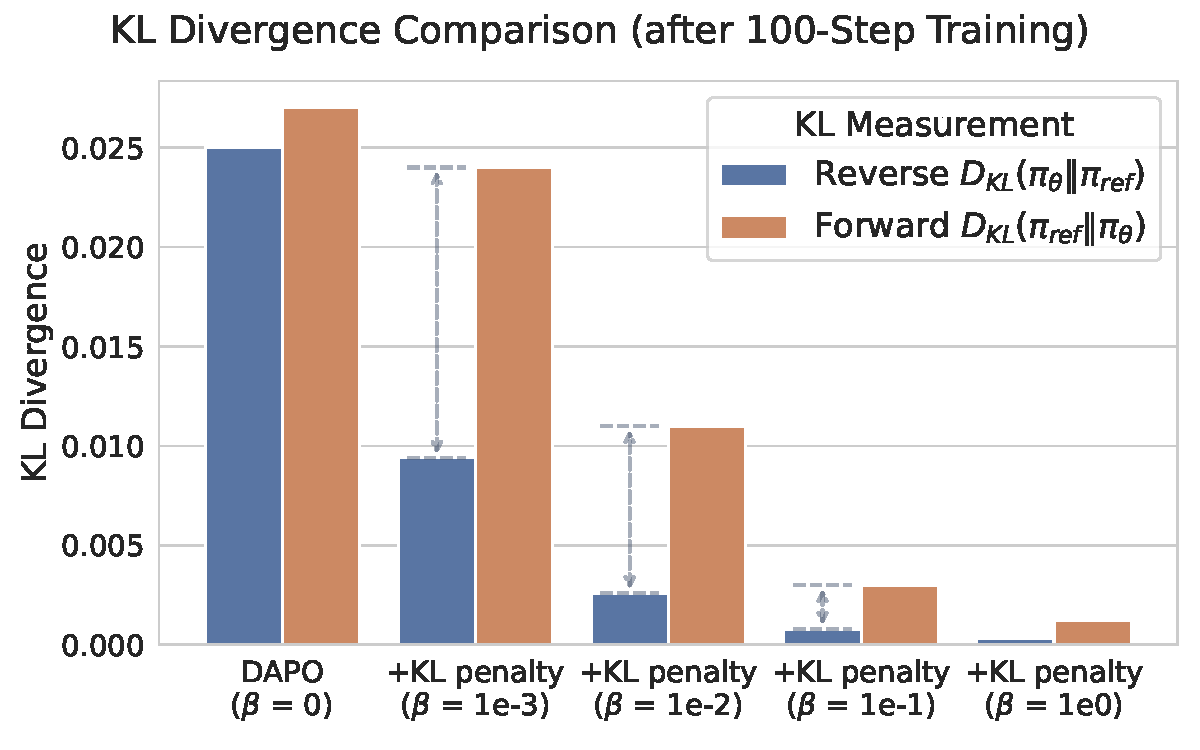
\includegraphics[width=\linewidth]{figs/kl_measurement.pdf}
        \caption{Reverse and forward KL measurements}
        \label{fig:kl_measure}
    \end{subfigure}
    \hfill
    \begin{subfigure}[b]{0.23\linewidth}
        \centering
        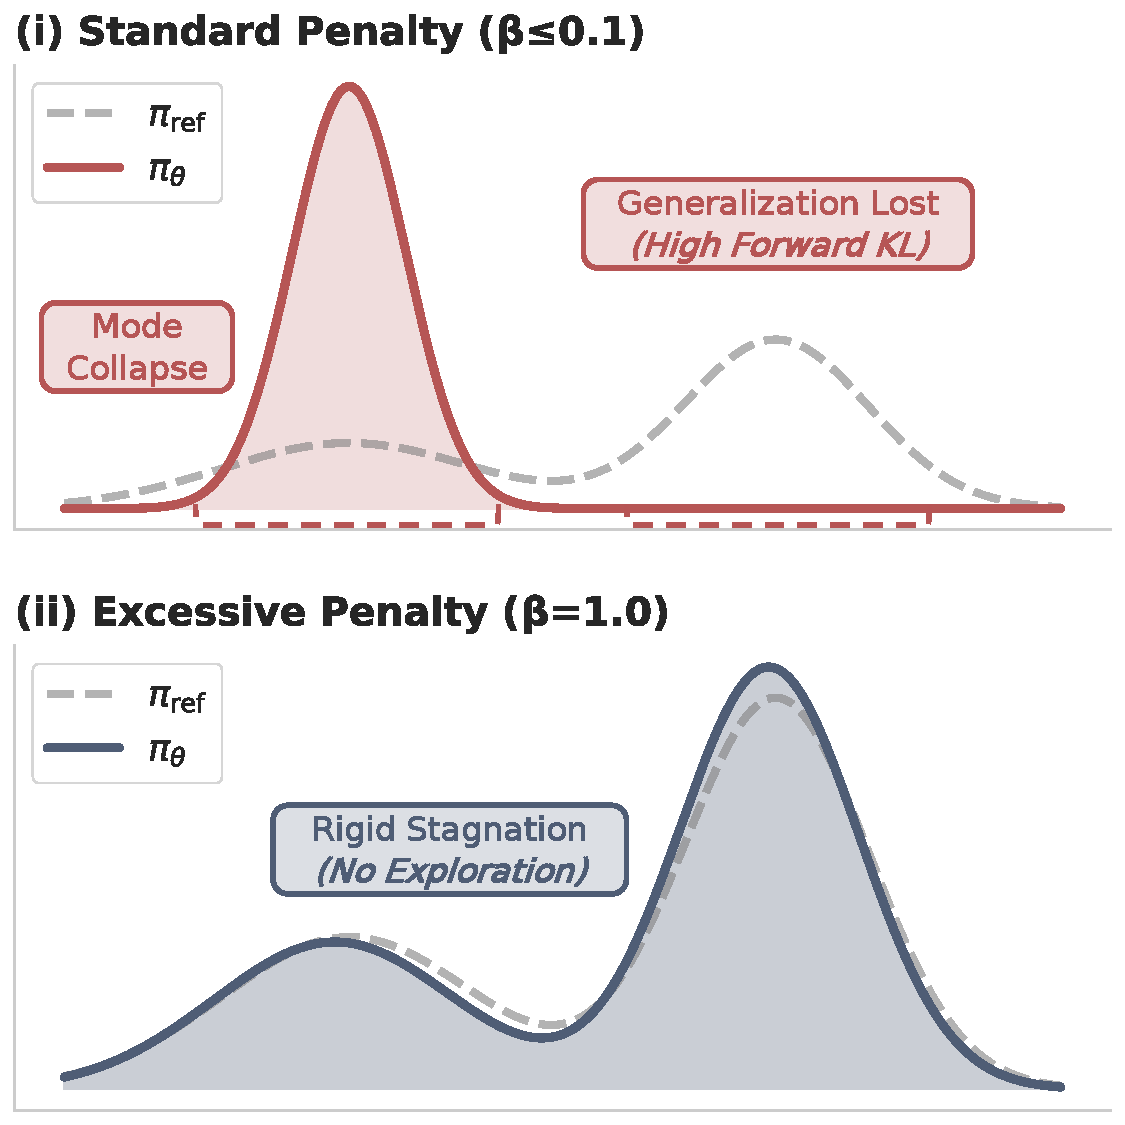
\includegraphics[width=\linewidth]{figs/kl_schematic.pdf}
        \caption{An illustrative example}
        \label{fig:kl_explain}
    \end{subfigure}
    \caption{(a) \textbf{Performance trends under KL regularization. }
    Standard penalties ($\beta \le 0.1$: \textcolor{myorange}{1e-3}, \textcolor{mygreen}{1e-2}, and \textcolor{myred}{1e-1}) merely delay validation collapse of the \textcolor{myblue}{baseline}, while the extreme setting (\textcolor{mypurple}{$\beta$ = 1.0}) ensures stability only by inducing stagnation, highlighting the stability-plasticity dilemma.
    (b) \textbf{Asymmetry in KL divergence} (measured after 100 steps of continual training).
    While increasing $\beta$ drastically reduces the optimized reverse KL $\mathbb D_\text{KL}(\pi_\theta\|\pi_\mathrm{ref})$, it is much less effective at constraining the forward KL $\mathbb D_\text{KL}(\pi_\mathrm{ref}\|\pi_\theta)$.
    (c) \textbf{An illustrative example}. 
    Standard penalties lead to mode collapse (indicated by high Forward KL) due to the mode-seeking nature of the objective, whereas excessive regularization suppresses the exploration required for learning.
    }
\end{figure*}

\noindent\textbf{KL Regularization}. 
Reverse KL regularization serves as the standard defense against over-optimization in RL training for LLMs \citep{klcomedy}.
Unlike early RLHF methods that apply KL as a reward penalty \citep{ouyang2022training}, reasoning tasks often adopt loss-level regularization to avoid penalizing response length \citep{GRPO}. 
We investigate two primary estimators for this term:
(1) The variance-reduced unbiased estimator (\texttt{k3}):
$\mathbb D_\mathrm{KL}(\pi_\theta\|\pi_\mathrm{ref}) = \frac{\pi_\text{ref}(\cdot)}{\pi_\theta(\cdot)}-\log\frac{\pi_\text{ref}(\cdot)}{\pi_\theta(\cdot)}-1$, which is used in GRPO;
and (2) the squared estimator (\texttt{k2}):
$\mathbb D_\mathrm{KL}(\pi_\theta\|\pi_\mathrm{ref}) = \frac12[\log{\pi_\text{ref}(\cdot)}-\log{\pi_\theta(\cdot)]^2}$, which is shown to provide unbiased gradients \citep{klpitfalls}. 
To ensure rigor, we empirically evaluate both estimators to determine if standard KL can bridge the generalization gap, with \texttt{k3} adopted for our main results and \texttt{k2} comparisons deferred to the Appendix.
% To ensure rigor, we empirically evaluate both estimators to determine if standard KL penalties can bridge the generalization gap, with \texttt{k3} utilized in our main experiments and the comparative analysis of \texttt{k2} provided in the Appendix.

% 在说明KL的计算的方式时，有几个要注意的地方
% 1. 为什么不用 KL in reward (ouyang2022)? 这里follow R1的做法，如果放到reward里面，所有token都累积惩罚，会导致直接惩罚长度
% 2. 为什么还要使用K2估计？根据kl pitfalls论文, k2估计优化的才是reversed KL, k3实际上优化了forward kl (但从结果来看，二者差不多）
% 3. 为什么用best ckpt作为ref？参考R1的做法，reference需要reset




\section{Empirical Analysis of KL Regularization}\label{sec:kl}

\textbf{Experiment Setup}.
To investigate the efficacy of KL regularization, we adopt a \textbf{continual training} setting focused on the phase where over-optimization emerges.
We first train Qwen2.5-Math-7B base model \citep{Qwen25Math} using DAPO to identify the peak checkpoint $\pi_\theta^*$ immediately prior to validation degradation.
We then resume training from $\pi_\theta^*$ under varying KL coefficients, aiming to turn around the degradation trend observed in the unregularized baseline.
In this phase, we set the reference policy to the current best model ($\pi_\text{ref} \leftarrow \pi_\theta^*$) rather than the initial base model.
This setup aligns with practical long-horizon RL training scenarios \citep{Deepseek-R1}, ensuring that the regularization term discourages deviation from the \textit{best-known} policy rather than enforcing regression to the weaker initial state\footnote{We also explored regularizing against the base model, but this led to rapid performance deterioration.}.

% \begin{figure}
%     \centering
%     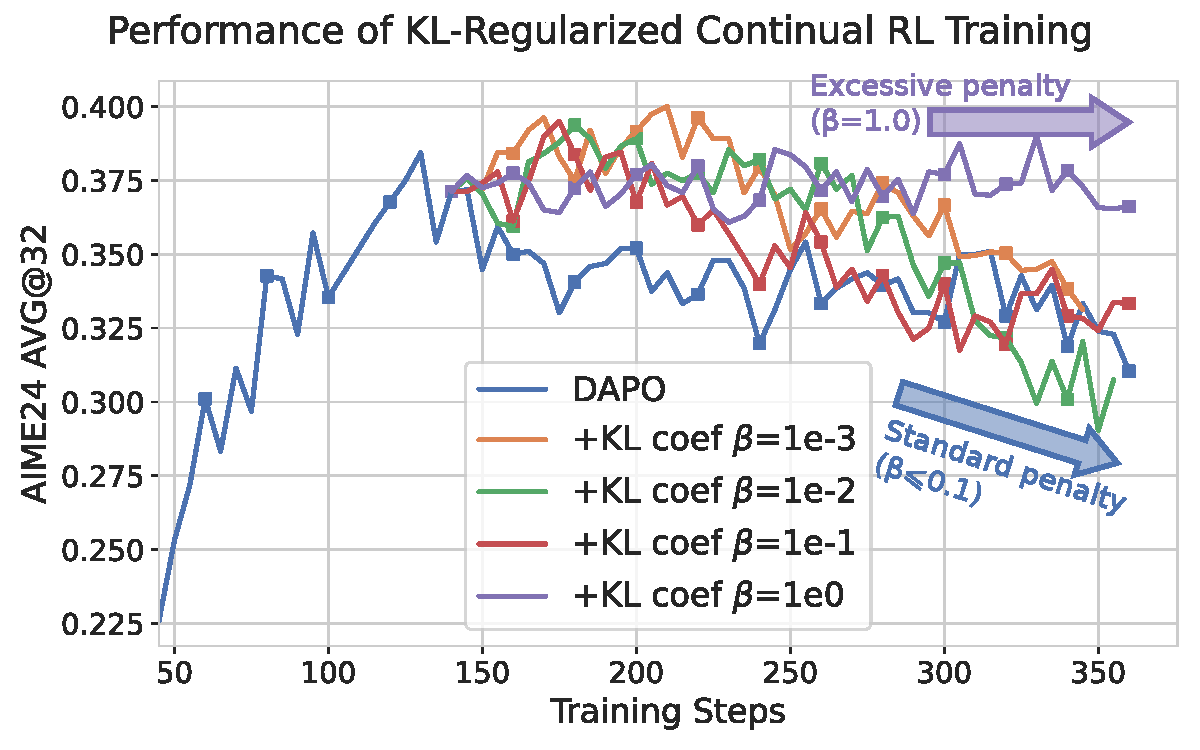
\includegraphics[width=0.8\linewidth]{figs/different_kl.pdf}
%     \caption{Performance trends under KL regularization. 
%     Standard penalties ($\beta \le 0.1$) merely delay validation collapse, while excessive regularization ($\beta = 1.0$) ensures stability but freezes performance (stagnation), illustrating the stability-plasticity dilemma.}
%     \label{fig:kl_perf}
% \end{figure}

\textbf{Evaluation Protocol}.
We evaluate reasoning performance on the challenging AIME24 benchmark and report \texttt{avg@k}, the average accuracy with $k=32$ responses sampled per question.
Beyond performance metric, we analyze distributional shifts by monitoring both the forward KL divergence $\mathbb D_\text{KL}(\pi_\text{ref}\|\pi_\theta)$ and the reverse KL divergence $\mathbb D_\text{KL}(\pi_\theta\|\pi_\text{ref})$.
Tracking both directions provides a holistic view of the policy drift: while reverse KL serves as the training penalty, forward KL offers deeper insights into whether the model maintains adequate coverage of the reference distribution.

\textbf{Empirical Results}.
As illustrated in Fig.~\ref{fig:kl_perf}, the unregularized baseline (DAPO) suffers from immediate degradation in validation performance as training proceeds.
Introducing KL penalties reveals a fundamental trade-off:

\textit{1) Standard Regime ($\beta \le 0.1$):} 
It is worth noting that standard RL practices typically employ minimal penalties\footnote{DeepSeek-R1 utilizes $\beta$=1e-3 \citep{Deepseek-R1}.}.
Even when increasing $\beta$ to $0.1$, the model eventually succumbs to \textbf{instability} after a brief period of improvement.

\textit{2) Excessive Regime ($\beta = 1.0$):} 
We further increase $\beta$ to $1.0$ as a stress test to probe the limits of regularization.
Although this extreme setting can suppress instability, it leads to \textbf{stagnation}.
This indicates that such stability is achieved only by rigidly tethering the policy, which precludes the exploration necessary for performance gains.

% \begin{itemize}[left=0.5em, topsep=0pt, itemsep=0pt]
% \item[(1)] \textbf{Standard Regime ($\beta \le 0.1$):} 
% It is worth noting that standard RL practices typically employ minimal penalties\footnote{For example, DeepSeek-R1 utilizes $\beta$=1e-3 \citep{Deepseek-R1}.}.
% Even when increasing $\beta$ to $0.1$, the model eventually succumbs to \textbf{instability} after a brief period of improvement.

% \item[(2)] \textbf{Excessive Regime ($\beta = 1.0$):} 
% We further increase $\beta$ to $1.0$ as a stress test to probe the limits of regularization.
% Although this extreme setting can suppress instability, it leads to \textbf{stagnation}.
% This indicates that such stability is achieved only by rigidly tethering the policy, which precludes the exploration necessary for performance gains.
% \end{itemize}

These observations hold consistently across both \texttt{k2} and \texttt{k3} estimators (\cf Appendix~\ref{appendix:add_exp}), indicating that reverse KL is insufficient for stable \emph{and} improving RL training.

% 这里的分析可以这样说：
% KL 约束太弱的时候，由于reverse KL mode seeking的特性， forward KL限制不住， mode collapse 仍然存在
% KL 约束太强的时候，由于 uniform penalty, 损害了模型优化的上限，根本就无法提升

\textbf{Analysis: Why KL Fails}.
To understand the mechanics of this failure, we examine the divergence metrics in Fig.~\ref{fig:kl_measure}. 
A clear \textbf{asymmetry} emerges:
while increasing $\beta$ drastically compresses the optimized reverse KL $\mathbb{D}_{\text{KL}}(\pi_\theta\|\pi_\text{ref})$, the forward KL $\mathbb{D}_{\text{KL}}(\pi_\text{ref}\|\pi_\theta)$ \emph{decreases at a much slower rate}, maintaining a disproportionately large gap.
This failure stems from two distinct mechanisms:

\textit{1) Mode-Seeking Nature (Standard Regime).} 
Under standard penalties, the optimization is dominated by the \textbf{mode-seeking nature} of reverse KL \citep{beyondkl,klcollapse}. 
Fundamentally, reverse KL only penalizes the policy for generating samples that are \textit{unlikely} under the reference distribution, but \textit{not} for missing valid regions of the reference support.
Consequently, the model can collapse onto a narrow subset of ``shortcut'' modes without incurring a high penalty, provided these modes exist within the reference distribution (as illustrated in Fig.~\ref{fig:kl_explain}).
This selective collapse discards other generalizable reasoning paths, resulting in the observed performance degradation and a much higher forward KL (which penalizes dropped modes).

\textit{2) Uniform Penalty (Excessive Regime).}
Under extreme penalties (\eg $\beta=1.0$), the regularization acts as a \textbf{uniform penalty} on all policy deviations.
While this forces $\mathbb{D}_{\text{KL}}(\pi_\theta\|\pi_\text{ref}) \to 0$ and thus locally aligns forward and reverse KL \citep{klpitfalls}, it indiscriminately suppresses both harmful degradation and beneficial exploration.
This causes the stagnation observed in our experiments, rendering the ineffective training.


\begin{paperbox}
Standard KL regularization faces a dilemma: loose constraints lead to \textbf{instability} due to its \textit{mode-seeking nature}, while tight constraints result in \textbf{stagnation} due to its \textit{uniform penalty}.
This analysis confirms that a passive penalty alone is structurally insufficient. 
\end{paperbox}
